
\chapter{Disaffirming the Myth of Dravidian-Aryan Divide Reaffirming Tamil Nadu as the Land of Dharma}

\Authorline{Shrinivas Tilak}


\section*{Introduction}

\vskip 7pt

As part of the Infinity Foundation (India)’s efforts to promote Indic thought and consciousness from a Dharmic perspective, the third Swadeshi Indology (SI-3) conference was held in IIT Madras from December 22-24, 2017 with the theme “Tamil Nadu—The Land of Dharma” emphasizing the state’s rich and varied contributions to Hindu Dharma, Sanskŗti, Itihāsa, and Paramparā. Padma Bhushan awardee Dr. Nagaswamy\index{Nagaswamy} (Founder, Tamil Nadu Archaeological Department), inaugurated the conference with an informative talk that drew out the similarities between the Sangam literary works and the Vedic texts. He explicitly showed how the Tirukkural,\index{Tirukkural} a famous fifth century work by the poet Tiruvalluvar,\index{Tiruvalluvar} is correlated with the Manusmŗti;\index{Manusmrti@Manusmŗti} concluding that the ancient Tamil text was inspired from the Dharmaśāstra of Manu. An enlightening panel discussion about the spiritual traditions of Tamil Nadu followed where speakers representing the Śaiva, Vaişņava, and Jaina traditions spoke about how their respective traditions or schools of thought flourished and coexisted in Tamil Nadu for thousands of years. The parting message and appeal of the conference for the delegates, the attendees, and the people of India on the whole was the need to \textit{reaffirm} Tamil Nadu as the “Land of Dharma” that remains in mutual harmony with the rest of the country. Though Āgama\index{Agama@Āgama} is (and has remained) the more dominant spiritual and social mode or stream of expressing Dharma in Tamil Nadu, it has also welcomed the various schools of thought belonging to Nigama,\index{Nigama} the other equally important spiritual social mode or stream of expressing Dharma. Āgama refers to the collection of practices and precepts (\textit{ācāra}-s and \textit{vicāra}-s) centered on the institution of \textit{pūjā} to Śiva, Vişņu and Devī preserved in the Kāvya and Śāstra types of texts in Tamil (and in Sanskrit). Nigama refers to collection of practices and precepts (\textit{ācāra}-s and \textit{vicāra}-s) centered on the institution of \textit{yajña} initially but subsequently extended to \textit{pūjā} to Vişņu and other Hindu deities preserved in Kāvya and Śāstra types of texts in Sanskrit (and some in Tamil).

\vskip 7pt

Another objective of SI-3 was to provide critical assessment of the Dravidian nationalist movements in contemporary Tamil Nadu known for their virulent attacks on Hindu Dharma using the caste system and the practice of untouchability\index{untouchability} as well as their penchant for Hindu-phobia. Participants who spoke on this topic pointed out that a strong anti-Hindu bias obtains in the Tamil and English print and visual media of today. Most young Tamils who enter university journalism departments or the media are already thoroughly ‘secularized’ and ‘westernized.’ The fact that most of them happen to be graduates of the English medium high schools operated by the Christian missions reinforces their anti-tradition and anti-Hindu stance. They are not trained to think and write about cultural, political, religious or social issues from an insider’s (i.e. an \textit{emic}) perspective. The humanities and social science departments of the universities they typically attend (Jawaharlal Nehru University, Delhi [JNU] for instance) are regrettably politicized where the search for truth is subordinated to left wing ideology. Commonly, graduates of these departments see Indic culture and society through an ideological prism of Marxism-Leninism and secularism that reinforces perceptions of Hindu dharma not on the basis of ‘objective’ observation and fact but on an ideological ground and emotion. There was general consensus at the conference that Dravidian nationalism that is now so rampant in today’s Tamil Nadu owes its roots to the Myth of the Dravidian-Aryan Divide\index{Myth of the Dravidian-Aryan Divide} that originated in the Aryan invasion (now described as ‘immigration’) theory which has remained a mainstream doctrine for more than a century.


\section*{Conference presentations}

In total forty-six papers were presented at SI-3 spreading across twelve sessions under the following themes: the Two spiritual streams of Dharma — Āgama and Nigama, Embedded Sacredness in Tamil Life; Modern Hinduphobia\index{Modern Hinduphobia} and Dravidian Movement;\index{Dravidian Movement} Caste, Untouchability and Hinduism; Roadmap for Future — Tamil Identity. The papers were selected after passing through double blind peer reviews, ten of which have been compiled in this volume. The papers call for a multidimensional approach in order to (1) disaffirm the Myth of Dravidian-Aryan Divide launched by the proponents of the AIT and (2) reaffirm the relation of harmony (\textit{samanvaya}\index{samanvaya@\textit{samanvaya}}) that traditionally existed between Tamil Nadu and the rest of India. Toward that objective they take a composite approach that is based on research in Kāvya, Śāstra, and \textit{Bhakti} texts in Sanskrit and Tamil combined with evidence from linguistics and numismatics. The papers generally follow the traditional debating format: ‘Pūrvapakşa-Uttarapakşa-Siddhānta’ (\textit{Arusamaya Pinakkam}). Pūrvapakşa ('the first side;' ‘\textit{Parapakka}’ in Tamil) is the technical term for the preliminary position, or prima facie view in a metaphysical or philosophical argument put forth in the form of an objection by the \textit{Pūrvapakşin} (opponent; real or imagined). The Uttarapakşa (\textit{Nirākaram}; also known as ‘\textit{Svapakka}’ in Tamil) refutes the argument put forth by the \textit{pūrvapakşin}. Siddhānta ('established end') is the technical term for the demonstrated and definitive conclusion of the debate.

\subsection*{Method of Samanvaya}

In the Indic tradition each Śāstra (science) has its own method (\textit{tantrayukti};\index{tantrayukti@\textit{tantrayukti}} \textit{tandiravutti}\index{tandiravutti@\textit{tandiravutti}} in Tamil), which is determined by the nature of that Śāstra. The subject matter of Vedānta (Adhyātmaśāstra), for instance, is \textit{brahman} and the method Vedānta adopts to establish its own understanding of \textit{brahman} is called \textit{samanvaya} meaning ‘coherence and harmony’ (internal and external unity respectively). If a text is meaningful in itself it is coherent. If that meaning is in agreement with other coherent texts, there is harmony. Analysis and interpretation proceed at two levels (\textit{anvaya-vyatireka}):\index{anvaya-vyatireka@\textit{anvaya-vyatireka}} emphasizing and establishing the non-dual nature of \textit{brahman}; i.e. what (and why) \textit{brahman is} (\textit{anvaya}) and refuting what (and why) \textit{brahman is not} (dual, phenomenal etc). In an extended sense \textit{anvaya} refers to the logical explanation of connection between words, ideas, or actions--as to how different words etc relate with each other to convey a significant meaning as between 'smoke' and 'fire.' It is universally known that "where there is smoke, there is fire." Traditionally, \textit{anvaya} is used along with the word \textit{vyatireka}, which means agreement in absence between two things, such as absence of 'smoke' and 'fire': "where there is no fire, there is no smoke." The method (\textit{yukti}) of \textit{samanvaya} thus is a method of synthesis and analysis, conjunction and disjunction. \textit{Anvaya/vyatireka} also constitutes a basic structure of Śankarācārya’s reasoning and method (\textit{yukti, tarka}, or \textit{anumāna}\index{anumana@\textit{anumāna}} in chapter eighteen of his Upadeśasahasrī.

Examination of a given topic of the Śāstra (\textit{adhikaraņa}) usually proceeds along the following steps: prima facie doubt or objection (Pūrvapakşa), reply (Uttarapakşa), and the conclusion (Siddhānta). The statement of the subject or the issue raised and the doubt or alternatives proposed constitute the context of the discussion (\textit{vişayo vişayaścaiva pūrvapakşas tathottaram nirņaya (samgati) śceti pańcāngam śāstre’dhikaraņam smŗtam})(Bhiksu Gaurisankara 1950: 11). \textit{Samanvaya}, then, may be understood as the Indic equivalent of hermeneutics used to interpret spiritual or philosophical texts (or topics) such as the Upanişad-s. As a method of harmonization, \textit{samanvaya} first occurs in chapter one of the Brahmasūtra,\index{Brahmasutra@Brahmasūtra} a text in four chapters wherein the author Bādarāyaņa reconciled and systematized the teachings of the Upanişads identifying a consistent set of doctrines running through them. It was through the instituted methodology of \textit{samanvaya} that the citizens of India grew up to be moderate, tolerant, and open minded with respect to diverse beliefs and practices. They were socialized to accept that the ability to tolerate each others' views enriched them and transformed them into a cultured individual (\textit{śişţa}). It is not that they did not realize what was untrue, but their focus was more on the aspects that \textit{were} true (see Brahmasūtra 1:1.1-4; \textit{tattu samanvayāt}).

Anthropologist Bronislaw Malinowski\index{Bronislaw Malinowski} reasoned that a scientific habit of mind is universal; that all people [cultures and societies] operate, or are capable of navigating through the domains of magic, science, and religion. In all societies (including Western civilization) practices dubbed ‘magical’ and ‘mystical’ coexist with rational/empirical processes. He was keenly alert to the double selection by which ‘primitive peoples’ are described entirely in terms of their mystical beliefs ignoring much of their empirical behavior in everyday life, while Europeans are described entirely in terms of scientific rational-logical thought (Tambiah 1990: 92). The method of \textit{samanvaya} gets away from this trap by maintaining that one can in a particular context operate in a transcendent or mystic mode and then can switch in another context to a practical empirical everyday frame of mind. Most modern scientists, however, are unwilling to make this concession.


\section*{I Pūrvapakşa: Imposing Dravidian and Aryan disharmony (\textit{duranvaya})}

\subsection*{The Aryan Invasion Theory (AIT)}

Nicholas Kazanas,\index{Nicholas Kazanas} Indologist and Director of Omilos Meleton Cultural Institute, Athens, examined the issues concerning the Aryan Invasion Theory and concluded that actual archaeological evidence and the Indo-Aryan documents are against the arrivals of ‘Aryans’ into India at about 1500 BCE as proposed in the Aryan Invasion Theory (AIT).\index{Aryan Invasion Theory (AIT)} The linguistic data used as evidence for the AIT can furnish no evidence at all either for the date of this entry or for the entry itself: in fact, they can be, and have been, interpreted quite differently. Recent genetic studies do not suggest any entry of Indo-Aryans in such numbers as would accomplish the full Aryanization of Saptasindhu and the farther North India within the last ten thousand years. Indeed all the data used as evidence by the AIT are wholly conjectural and arbitrary and often consist of misrepresentations and distortions (Kazanas 2006). American archaeologist J. Shaffer had the courage to call the AIT of India "a myth." The development of this "myth" which had obtained mainstream status in academia is well traced by Edwin Bryant. Having started as a linguistic theory, it later acquired biological undertones involving more or less obvious ethnic/racial prejudices (Bryant 2001, Shaffer 1984; cited in Kazanas 2006). Kazanas explains how, before the Nazi “aryanism” of the 1930’s, the AIT was used by colonial politics as is obvious in the speech of British Prime minister Stanley Baldwin (cousin of Rudyard Kipling) in Parliament in 1929:

\begin{myquote}
Now after ages... the two branches of the Aryan ancestry have again been brought together by Providence... By establishing British rule in India, God said to the British, ‘I have brought you and the Indians together after a long separation... it is your duty to raise them to your level as quickly as possible... brothers that you are’”! God’s ways were no longer so mysterious (Kazanas 2006). 
\end{myquote}



\section*{Myth of Dravidian-Aryan Divide}

The Myth of Dravidian-Aryan Divide\index{Myth of Dravidian-Aryan Divide} (hereafter Myth) continues in the West and among Indian academics because vested’ interests and academic posts are still involved and will continue to be involved because the human ego is not educated to let go of claims that are shown to be untrue. E. Leach pointed out (1990), academic posts and reputations are involved. Scholars are people and people tend to be attached to and identified with their ideas, posts and reputations (and incomes). Consequently they persist with their models and paradigms irrespective of other factors. In Indology and Indo-European studies the mainstream orthodoxy, despite the preceding evidence, will not allow the case for ‘Out of India’ theory and a time period when the Ŗgveda\index{Rgveda@Ŗgveda} was compiled in the 4th millennium BCE to appear in any form in the media it commands. Michael Witzel\index{Michael Witzel}, for instance, observed: “It is certain that Kazanas, now that he is published in JIES, will be quoted endlessly by Indian fundamentalists and nationalists as ‘a respected scholar published in major peer reviewed journals like JIES’ — no matter how absurd his claims are known to be by specialist readers of those Journals” (2003: 23, §5 end; Kazanas 2006).

\subsection*{Rajiv Malhotra and Aravindan Neelakandan on the Myth of Dravidian-Aryan Divide:}

Presenters at SI-3 demonstrated keen awareness that disaffirmation of the Myth of the Dravidian-Aryan Divide and correct comprehension of the AIT (its driving motor) by the people of India is critical in the fight against the ‘breaking India’ forces so forcefully argued and meticulously documented by Rajiv Malhotra\index{Rajiv Malhotra} and Aravindan Neelakandan\index{Aravindan Neelakandan} (M\&N) in their masterpiece monograph \textit{Breaking India: Western Interventions in Dravidian and Dalit Faultlines} (BI; 2011). Starting from an analysis and discussion of the European Race theories, the Aryan invention, Imperial evangelism, and the “caste” construction, M\&N focus on Dravidian and Dalit identity\index{Dalit identity} separatism that is being fostered by the Christian West in India the name of human rights. The first half of BI documents how Aryan theory was fabricated in the workshops of European evangelists and Indologists and how deeply it has affected the Indian mindset; how social principle of the division of labor (\textit{varņa}) was transformed into a nasty nexus of “the caste system.” From the “Myth of Ham” European and British evangelicals justified their claim that labor of all Native Americans, Africans, and Indians may be freely used because they all are sons of Ham. In the second half of the book M\&N discuss the digestion of Hindu dharma into Dravidian Christianity and the more recent phenomena of the Afro-Dalits. The thesis of BI may be summarized as follows:

\subsubsection*{I Distorting categories of ‘Aryan,’ ‘Dravidian,’ and Tamil}

Presentations at SI-3 began with the Pūrvapakşa by insisting that the very idea of there being a distinct and separate linguistic, cultural, and ethnic Dravidian identity took root only after the AIT gained a firm foothold in India. The Brahmins subsequently began to be projected as a foreign ‘Aryan’ race who purportedly arrived south in Tamil Nadu and introduced a religion which now goes by the name ‘Hinduism.’

\begin{myquote}
... the Vedas belonged to the foreign Aryans, who were pure, while the modern Hindus were degenerate bastard off-springs of these White Aryans mating with the inferior Dravidian natives. However, the Dravidians were now being given their own glorious past with their origins in Lemuria\index{Lemuria} (Malhotra and Neelakandan 2011: 82).
\end{myquote}

The Dravidianists\index{Dravidianists} now began to propose that Brahmins, Sanskrit and Vedānta were evil forces that needed to be eradicated to re-purify Tamil Society (Malhotra and Neelakandan 2011:97). In the early 20th century, an anti-Brahmin political organization called the Justice Party was started, which in 1944 was renamed ‘Draviḍar Kaļagam’\index{Dravidar Kalagam@Draviḍar Kaļagam} (a social organization) under the leadership of ‘Periyar’ E. V. Ramasamy. Since then, the various Dravidian Parties (including the Draviḍa Munnetra Kaļagam\index{Dravida Munnetra Kalagam@Draviḍa Munnetra Kaļagam} = DMK; the political offshoot of the Draviḍar Kaļagam) have held Tamil Nadu in their ideological sway for over half a century. The distorted and contorted manner in which the equation Aryan=Brahmin=Hindu is posited continues to feed the divisive politics at all levels in Tamil Nadu. Proponents of the AIT decisively split Indian languages into two global language ‘families: the Aryan (later redubbed Indo-European) family pertaining to North India, and the newly certified Dravidian family, with Tamil as its fount, pertaining to India South of the Vindhya mountains. The conflation of linguistic ‘family separation’ with ‘racial’ separation was actively pursued without mentioning it formally. Strenuous efforts were (and still are) made in mainstream scholarship to show that the so-called indigenous Dravidians occupied the whole of the subcontinent and beyond — as far as the Middle East.


\subsubsection*{II Sowing disharmony (duranvaya) between ‘Dravidians’ and ‘Aryans’ }

\begin{myquote}
Bishop Caldwell proposed that the Dravidians were in India before the Aryans, but got cheated by the Brahmins, who were the cunning agents of the Aryans. He argued that the simple-minded Dravidians were kept in shackles by Aryans through the exploitation of religion. Thus, the Dravidians needed to be liberated by Europeans like him. He proposed the complete removal of Sanskrit words from Tamil” (Malhotra and Neelakandan 2011: 62).
\end{myquote}

Caldwell thus divided Indians linguistically and religiously and established the theological foundation for Dravidian separatism from the pan-Indian Dharma. The word ‘Draviḍa’ came into popular use to denote the people of non-Brahmin class belonging to the Kerala, Karnataka, Andhra and Tamil Nadu regions of South India was in 1912 with the formation of the ‘Draviḍa Association.’ It adopted the name ‘Draviḍa’ from an earlier group that called itself -\textit{Dravida Jana Sabha}. This was an important tipping point in the history of Dravidian nationalist movement, which began to declare itself as the custodian of ‘\textit{Dravida}’ interests. Later, DMK inherited its policies from the Draviḍa Kaļagam, which came into being when caste divide in the society had reached its zenith. The era of Indian independence coincided with this context and many leaders emerged who gave vent of this oppressive climate. One of them was E. V. Ramasamy\index{E. V. Ramasamy} Naicker (1879-1973; EVR). Due to his early experiences in life of caste divisions and separation, he was against the Brahmin class and the importance given to this section of society in social, religious and political context. He also propagated the self-respect movement in 1925 which demanded equality for all classes in the society and encouraged backward classes to command self-respect in a caste-based hierarchical society. EVR shaped the Dravidian social movement’s focus of recognizing the Brahmins as the real threat rather than the British who ruled India then. He called his fellow men to establish equality with Brahmins before they sought equality with foreigners.

Under M. Karunanidhi (1924–2018), DMK executed what EVR had envisaged — wiping out the collective memory of the Brahmin community in Tamil Nadu which was accomplished by institutionalizing the theory of Dravidian-Aryan Divide. Over time, however, M. Karunanidhi\index{M. Karunanidhi} and DMK realized that their atheist beliefs were not popular with the majority in Tamil Nadu. The majority of the society found succor in following their beliefs in traditions and customs of religion. Recognizing the trend, they tried to rebrand DMK as the flag bearer of caste equality and decided to associate DMK with Rāmānuja,\index{Ramanuja@Rāmānuja} the patron saint of Brahmin community seen by all as a saintly person who strived for everyone’s spiritual liberation beyond all differences in castes, gender, etc.


\subsubsection*{III Constructing a de-Indianized Christian ‘Dravidian’ identity }

Chapter six of BI elucidates ongoing de-Indianization of the Tamil tradition, culture, and society that began with Bishop Robert Caldwell (1814-1891), an evangelist for the society for the propagation of the gospel, who actually came up with the idea of a ‘Tamilian’ Dravidian race. Another missionary Indologist George U. Pope\index{George U. Pope} (1820-1908) played a lead role in claiming Tamil classical literature to be un-Indian, un-Hindu linking it to Christianity. A Conspiracy theory was propagated to stress the cunning Aryans and Brahmins exploiting innocent Dravidians. Initially, it was Christian missionaries — operating mainly in and around the southern coastline of India between Madras \& Cochin that sold to the local populace, the narrative of a Christian Dravidian identity.\index{Christian Dravidian identity} A case in point would be the mapping of the epitome of Tamil-Hindu classic text \textit{Tirukkural}\index{Tirukkural@\textit{Tirukkural}} onto Christianity. Today, Dravidian politics and the Dravidian Christianity movement continue to be the primary proponents of the debunked Aryan Invasion theory. For example, there have been attempts to delink Tamils from Hinduism ever since the British colonial era.

\begin{myquote}
“The missionaries’ strategy was two-pronged: First, they intensely studied the devotional Tamil literature and praised it in glowing terms to Tamil scholars. Second, they projected the Tamil culture as being very different and totally independent from the rest of India. Their work provided the ideological underpinnings of later Tamil racist politics. Missionary scholarship stimulated a new local ethnic identity, which was instructed to reject its Hindu nature. It became strategic to show that Tamil religion had strong underpinnings, on par with ‘civilized’ religions, and that ‘civilized’ meant monotheistic. These positive features were isolated and claimed to be indigenous to the Tamils, and shown to be in opposition to the ‘foreign’ traits that were attributed to the Aryans” (Malhotra, Neelakandan 2011: 65).
\end{myquote}


\subsubsection*{IV Digesting dharma into Christianized Dravidian identity}

Chapters eight and nine of BI elucidate how Hindu dharma is being digested into ‘Dravidian’ Christianity using the Myth of St Thomas. Evangelism is harnessed in the cause of the Dravidian Movement and to Christianize elements of Hindu popular culture such as the Bharatanāṭyam.\index{Bharatanatyam@Bharatanāṭyam} The proponents of the Myth initially recruited the colonial administrative officials who also doubled as Orientalists to come up with a compelling “Dravidian Proof.” Subsequently, European and American academic networks were recruited to perpetuate the Myth (BI Fig~10.1). These networks quickly established control over social discourse and gaze using philology, anthropology, and exegesis to proclaim existence of a distinct Tamil linguistics and to separate Aryan and Dravidian grammars. Yale University, for instance, sponsored the Dravidian etymological dictionary; while at Harvard University, Dravidian antiquity and Aryan borrowing from the Tamil classical literature was promoted. It was also projected as ‘secular’ and ‘un-Indian. Elsewhere at American universities, art and cultural studies of South India are pushed and in courses on anthropology of caste (\textit{jāti}-s) are equated with \textit{varņa} positing the caste system as uniquely a Hindu problem; absolving other Indian religions and social systems and cultures of other countries of this problem. A seminar on ‘Dravidian Religion to eradicate casteism was held in 2000 and in 2001 India was declared the ‘Mother of International Racism.’ At a conference in New York, Hinduism was‘re-imagined’ to be St Thomas Dravidian Christianity and Dravidian Christianity became an international movement. 2007 saw Second International Conference on the History of Early Christianity in India and in 2008 First International Conference on the Religion of Tamils was held. The salient features of the breaking India forces addressed in BI are provided schematically in the \textbf{Appendix}.


\subsection*{Divide, Digest, and Demonize}

M\&N argue that appeasing the Dalits (or the Christians for that matter) in India as minorities by conferring upon them special rights and privileges in order to promote social peace or harmony is really paving the way for India’s disintegration. Sri Sri Ravi Shankar (who heads the \textit{Art of Living Foundation} in India with branches all over the world) supports M \& N on this point. In an article published in \textit{The Times of India} (November 5, 2005; Pune edition), he criticized the actions of Dalit leaders like Kancha Ilaiah who took the issue of discrimination against the Dalits and deprivation of their human rights in India to the United States Congress. In the name of Dalit upliftment, Shankar argued, they were pursuing an ideological agenda and damaging the image of the country. “If they were really interested in the betterment of the Dalits, they should work in the villages in India instead of going to the US Congress,” argued Shankar. Kancha Ilaiah and company would do well to learn a thing or two from the [accursed] Yankees: national pride. There are three million homeless beggars in America, a little over one percent of the population. Yet, the American media generally does not publicize this fact abroad and, on the whole, American blacks have not asked the United Nations or any another country to interfere in the internal matters of the United States on their behalf (Ravi Shankar 2005).

François Gautier, a French journalist now based in India, notes that although most of intellectual elite of Tamil Nadu is born Hindu, the great majority of them are Hindu haters that are ashamed to identify themselves as Hindu. Their reports always come out sprinkled with the same clichés to slam Hindu dharma and Hindutva: the Saffron Brigade, the Hindu fundamentalists, fanatics, fascists, or communalists (Gautier 2002). \textit{Courier International}, a prestigious French magazine, which is read by diplomats and politicians, published a special issue on ‘Hindu fundamentalism’ with a cover photo of the RSS members doing their drill holding a wooden staff. The ignorant Westerner who read it, goes on Gautier to say, must have had the impression that India indeed is in the grip of fascist, Nazi-like Hindu groups where civil liberties are curtailed. When the editor-in-chief of that magazine was contacted, he pointed out that all the pieces had been translated from articles written in the Indian Press by Indian journalists. “If I did not know India,” wrote Gautier in one of his other writings, “I would tend also to believe what I read about India in the Western press: a nation torn by caste discrimination, and Hindu extremism. But after living more than thirty years in this country, my experience is totally different: Hindus are probably the most tolerant people in the world” (Gautier 2002)


\section*{II Uttarapakşa: Affirming Draviḍa - Ārya harmony (\textit{samanvaya})}

\subsection*{Cut the funk: take guard on the Kurukşetra}

The presentation of the Pūrvapakşa using insights from BI illustrates the sinister nature of the threats posed to Indic civilization. The elaborate machinations of expansionist Western civilization are ever present albeit in a different \textit{avatāra}. They continue to operate using the mechanisms provided by “modernity”—such as the academia, capitalism, and their likes. It is up to intellectuals and thought leaders to understand the true nature of the systems, processes operating around us and understand their motives and mechanisms. The nature of the Kurukşetra is that the ‘breaking India’ forces originating from the Myth of Dravidian-Aryan Divide\index{Myth of Dravidian-Aryan Divide} have to be confronted simultaneously on all fronts. Another important point to note is that not one of the ideologies behind the Myth was or is developed indigenously (i.e. Swadeshi); they are all Videshi.

M\&N do not mince words when they explain how Western interventions utilize and deepen Dravidian and Dalit fault lines for their plans to break India apart. They spell out in detail how a great deal of separatism in contemporary India is rooted in the Aryan invasion/migration (AIT/AMT)\index{Aryan invasion/migration (AIT/AMT)} theory. The modern South Indian political identity and vote banking has been driven on such assumptions. The Church has appropriated these fragments and is trying to unify them under the roof of Christianity by fabricating the history of Tamils and others in a pro-Christian manner. Thus this is not only an academic issue; it also has become a political issue (see Rajiv Malhotra’s e-mail interview with ‘Sandeep’ published on May 25, 2011 \url{www.sandeepweb.com}).

The guiding message that M\&N bring to Hindus in India therefore is: “Cut the funk; take guard on the Kuruksetra.” So what is \textit{funk}? An anecdote may be relevant here: A gentleman goes to a book store in Pune owned and operated by a Muslim. As he is browsing, the owner asks him "Are you Muslim?" "Ye....s," replies the gentleman sheepishly," and a Christian, and a Buddhist and a J..." "stop, stop" interjects the exasperated owner. "I know who you really are; you are a Hindu!" "Yes, I’m" came the confession eventually. Professor Dad Prithipaul (born of Hindu parents in Fiji), a retired professor of Hinduism from University of Alberta, Edmonton, Canada, has called this form of Hindu hiding (or denial) of self identity 'funk' (from Flemish \textit{fonck} = terror, panic, fear). The educated Hindu of today (writes Prithipaul) has to overcome an inner resistance when the occasion requires him to say: “I am a Hindu” as a noun or “I am Hindu” as an adjective. He is afraid to say it or to own it. The funk which inhabits his consciousness is evident when he hastens to qualify his Hinduness with a ‘but’ when he sets forth the damper: “I am a Hindu, \textit{but} I am a universalist/Indian first.” In the West it would be rare to hear someone proclaiming “I am Christian, but I am a Canadian, or a Frenchman, or an American first” (see Prithipaul 2005).


\subsection*{Refuting the Myth of Dravidian-Aryan Divide\index{Myth of Dravidian-Aryan Divide}}

Presentations at SI-3 conference in Chennai marshaled impressive evidence by way of Uttarapakşa to disprove the distorted versions of the categories of Aryan, Dravidian, and Tamil outlined in their presentations of the Pūrvapakşa. Attention was drawn to the fact that the AIT has not found scientific traction based on archeological, genetic or literary hard data. There is no physical evidence of an invasion followed by mass annihilation and/or exodus. Secondly, there is no evidence to show any form of genetically distinct identities, viz., Dravidian and Aryan, in the subcontinent. India’s population mix has been stable with no evidence of Central Asian gene influx for the past ten thousand years. Finally, there is no literary reference to any invasion and subjugation either by the (supposed) invader or by the invaded peoples. Next, there is no reference to the areas of the subcontinent from which the Aryans are accused of having pushed away the Dravidians. On the other hand, the word ‘Aryan’ and several of its variants are seen in the Tamil Sangam literature (dated to have begun in the 3rd century BCE) over several centuries but none of the multiple usages has any racial/cultural implication. This is in stark contrast to the common references to the Bauddhas and the Samanas (Jainas) as distinct (sometimes hostile) Dharmic communities in these works as well as in inscriptions. An occurrence of such magnitude as the Aryan Invasion — which is purported to have turned topsy-turvy the social and political equations — is mentioned in none of the earliest Tamil works which is concrete proof that it never occurred in the first place. Furthermore, there is no reference to any such invasion in any of the literary or oral traditions of the outsiders while referring to the Aryans and the Dravidians.

Ancient Tamil society was categorized into four traditions followed by people: Arasar (also Āndār), Antanar, Vaigar and Vellālar, which correspond to Kşatriya, Brāhmaņa, Vaiśya and Śūdra respectively. Tolkappiar describes Antanar as the one with the thread, the \textit{kamaņḍalu}, the \textit{tridaņḍa} and the wooden seat. An identical description of Antanar is found in Ettutogai. Similarly, descriptions of each of the other three traditions and their lifestyles are also described in detail by Tolkappiar. Interestingly, the Tamil word ‘varuṇanai’ (meaning ‘to describe’), is akin to the Sanskrit word ‘\textit{varņa}’ which means ‘to ‘sort out.’ ‘Vaņņathar’ (which could also mean ‘coloring people;’ i.e. dyers of cloth, in its more common usage) is clearly depicted as ‘people of specific qualities’ in the Sangam Literature. From the above, it seems obvious that the \textit{varņa} system existed in Tamil Nadu from very early times and was well-established when Tolkappiar alluded to it and that the social structure was akin to the non-Tamil societies of the sub-continent. There was no racial or ethnic association with any of the \textit{varņa-}s. All of them were perceived and treated as part of the society. There is no association of skin colour to classify the \textit{varņa}-s, as is interpreted by the proponents of the Aryan Invasion and Southward Expansion Theory. The Dravidianists’\index{Dravidianists} restriction to only two kinds of people--the Aryans who are Brahmins and the Dravidians who are not Brahmins does not account for the other two \textit{varņa}-s of the society (Joshi and Harshavardhana 2017).


\subsection*{Draviḍa, Ārya, and Tamil}

In his \textit{Tathyadarśana}, Sediyapu Krishna Bhat (1997) discussed the Dravidian-Aryan issue at length from the viewpoint of linguistics. Analyzing the meaning of the word \textit{draviḍa}, Sediyapu refuted the claims made about ‘Dravidians’ by Robert Caldwell. Before the nineteenth century, i.e. before Western scholars misrepresented it, the word \textit{draviḍa} only meant the Tamil language. Its etymological derivation can be explained in the following way: \textit{dru} (\textit{nāmapada}) + \textit{ila} (\textit{taddhita-pratyaya}) = \textit{dravila}. As per the famous rule ‘\textit{ḍalayorabhedaḥ},’ \textit{dravila} becomes \textit{draviḍa}. The \textit{nāmapada ‘dru’} means a tree. The \textit{taddhita-pratyaya ‘ila’} literally means ‘filled with’ – for example, \textit{phenila = phena} (foam) + \textit{ila}, means, ‘filled with foam.’ Hence, the meaning of \textit{dravila} is, ‘filled with forests trees’—i.e. a land filled with forests—Western Ghats, Eastern Ghats and Nilgiris—which corresponds to South India and specifically Tamil Nadu. In those days, Kerala was not an independent state; it was a part of Tamil Nadu as the Cera\index{Cera} province. Therefore, all the three mountain ranges were housed in Tamil Nadu. This is supported by \textit{kuriñji-tiṇai} in \textit{Tolkāppiyam,}\index{Tolkappiyam@\textit{Tolkāppiyam,}} known for its mountain slopes occupied by dense forests. Draviḍa thus suggests a wider term which includes (but is not exclusive to) the Tamils. Presently, however, the Dravidian ideologies are popular more in Tamil Nadu than elsewhere in the southern regions of India (see Krishna Bhat cited in Ganesh and Shashi Kiran 2017).

Kannada scholar S. Srikant Sastri has noted that the word ‘Draviḍa’ is absent in Sangam\index{Sangam} literature; nor is it seen in any of its variants--‘dravidar,’ ‘draviḍai,’ or ‘draviḍam.’ ‘Draviḍa’ itself is not of Tamil origin and Tamil grammar does not provide for two of the sounds in the word: First, no word begins with a sonant and so cannot begin with ‘d.’ Second, no word begins with a half-syllable. The word Draviḍa therefore must have originated outside of Tamil, most likely Prakrit or Sanskrit, in order to refer to the people in the Southern parts of the subcontinent. The very first use of the word ‘Draviḍa’ in Tamil to refer to the Tamil language is made by the great yogi Tāyumānavar, in the 18th century. The variants of the word ‘Tamila’ (Tamilian) such as ‘Damila’, ‘Dramila’, ‘Tamira’ and so on have been used by others to refer to the Tamils )(S. Srikant Sastri in Ganesh and Shashi Kiran 2017).

Analyzing the etymological meaning of the Sanskrit word ‘\textit{ārya},’ Sastri explained that it is derived from the root “\textit{ṝ – karṣaṇe},” which means, ‘to plough,’ ‘to cultivate.’ He posited that Aryans were originally an agricultural people and not a primitive marauding warrior-folk in the pastoral stage of civilization. Sastri affirmed that the theory of autochthonous origin of the Aryans in India cannot be dismissed as an expression of Hindu chauvinism, as it is the only theory consistent with available evidence. Drawing from the vast Vedic lore, he showed how the Aryan homeland is primarily Brahmāvarta (Eastern Punjab) and Brahmarṣideśa (Ganga-Yamuna doab). These were the centers from which Vedic speech and culture migrated to the west, east, and the south in the early Paleolithic period. In this regard, he pointed at the fact that the \textit{Ṛgveda} knows only of the land of the \textit{sapta-sindhu} and the most sacred place is Brahmāvarta bound by Dṛśadvatī and Sarasvatī (\textit{Ŗgveda}. 3.23.4)(see S. Srikant Sastri in Ganesh and Shashi Kiran 2017).

The word ‘āriyan’ and its variants, ‘āriyam,’ ‘āriya,’ and ‘āriyar’ are seen in Tamil literature right from the most ancient Sangam literature. In the other Sangam literary works, including Aganānūru and Puranānūru, the word ‘āriyan’ has been used in various contextual meanings including ‘northern king,’ ‘those living in the Himalayas,’ ‘rishis from the snowy mountains (Krishna Bhat in Ganesh and Shashi Kiran 2017). In such usages, the word denotes one who was from a part of the subcontinent which was not native to the Tamils, and nothing therein indicates anything racial either explicitly or implicitly. Jha notes that the sound systems of Indian languages across families show remarkable similarity in terms of vowel and consonant systems, syllable structure and the \textit{sandhi} formation. There are many features shared between the dominant families of India.” He therefore does not rule out the possibility of “a common origin for so-called Indo-Aryan and Dravidian languages (Jha 2013: 35).


\section*{Essays in this collection}

The collection opens with the essay by Ravi Joshi and Yamuna Harshavardhana in which the two authors set out the task of disaffirming the Myth of Dravidian-Aryan Divide by challenging the deeply contentious AIT theory (along with its very questionable methodology) by examining and critiquing the writings of (1) George L. Hart (Professor of Tamil language at the University of California, Berkeley), (2) Robert E. Frykenburg\index{Robert E. Frykenburg} (Professor of History and South Asian Studies, University of Wisconsin-Madison), and (3) E.V. Ramasamy Naicker. The authors bring out the internal differences between Tamil Nadu on the one hand and the modern states of Karnataka/Andhra, and Kerala on the other in order to argue that no ‘homogeneous’ thing as “Dravidian” covering the entire South of India existed as claimed by Dravidian nationalists. Based on insights of Ananda Coomaraswamy and M.N. Srinivas, they explain why the \textit{emic} explanatory mode is more suitable for interpreting the data on Tamil Sanskrit interactions than Western Indology’s fixative \textit{etic} mode that concentrates on the origins and priority (who came first, who copied from whom), and on Manichean narrative of two utterly independent well developed entities –Dravidians and Aryans interacting in a way full of friction and conflicts. Any serious observer of Indic history knows this is far from true, and that the mutually respectful interaction between the Sanskritized world with its surroundings – including the ‘tribal’ forest cultures and ‘Dravidian’ South – was a model successfully and peacefully replicated over and again in the history of India until the advent of Islamic conquest and British Imperialism. Using G Srinivas Reddy's work (Reddy 2011) on the historical interpretation of Krishnadeva Raya’s literary masterwork, the Amuktamalyada, Joshi and Harshavardhana show two-way North-South interactions, and the deep layout of Telugu Kannada world exemplified by the Vijayanagara\index{Vijayanagara} Empire with its overall Dharmic emphasis, contrasting wherever required with the empire’s pragmatic use of “mleccha” men, materials and ideas. This is a demonstration of the natural Indic Dharmic tendency to respond constructively to social change, based on a millennium of North South mutually respectful 'blending' (i.e. \textit{samanvaya}) The authors also bring out a detailed picture of a cultural zone that acted as a 'grey area' between the Northern and Southern expressions of Indic culture. Its existence, they argue, belies the Dravidian nationalists’ claim of a sharp South- North cultural divide. Emically speaking, Indic Civilization has had two major Dhārmic loci\index{Dharmic loci@Dhārmic loci}—(1) in the Sanskritic/Vedic/yogic basis originating in North India and (2) the Tamil/Vedic/Āgamic/siddhār basis originating in South India. The composite and pluralistic nature of the Indic civilization, they conclude, allowed for free mutually respectful exchanges between these two major cultural zones over millennia.

The next essay by Manogna Sastry and Megh Kalyanasundaram begins by observing that the Myth of Dravidian-Aryan Divide\index{Myth of Dravidian-Aryan Divide} and the AIT literally took away the proverbial home-ground of the Indians and everything that is India’s original contribution to the world knowledge systems. Being restricted to a model of language relationships and of linguistic descent the AIT tells us nothing certain about the origin of the Indic civilization. Taking a multi-disciplinary approach (rather than solely relying on linguistics as Western Indologists do), they analyze thirteen key indigenous sources identifying over two hundred occurrences of the terms Ārya and Draviḍa in order to rebut the Pūrvapakśa of Indo-European (IE) linguistics from an insider’s (emic) perspective. Sastry and Meghasundaram found no references to the word \textit{dravida} in any of the three books of the \textit{Tolkāppiyam}\index{Tolkappiyam@\textit{Tolkāppiyam}}—the \textit{Ezhuttadikaram}, the \textit{Solladikaram} and the \textit{Poruladikaram}—the oldest surviving work on Tamil grammar, literature and linguistics. Neither did they find references to the term in \textit{Srimad Bhagavatpurāṇa}, Kālidāsa’s\index{Kalidasa@Kālidāsa} \textit{Abhijñānaśakuntalam, Raghuvaṃśam} nor in \textit{Kumārasaṃbhavam}. In the many references to the occurrences of the terms in the \textit{Mahābhārata}, they were led to the same conclusion.

Consequently, the two authors find no basis for an ‘Aryan’ invasion/ migration into India accompanied with import of Sanskrit and Ŗgveda and no evidence for ‘Aryan’ anywhere in the world (of course, prior to formulation of AIT), which leads them to posit that (1)‘Sanskrit’ language (or its ‘precursor) as well as ‘Sanskrit’ language-based culture existed in India long before 2000 BCE; (2) the word ‘Aryan’ itself was a confused derivation of a similar word that existed in India, long before 2000 BCE.; and (3) Ŗgveda\index{Rgveda@Ŗgveda} –the oldest available text of humanity, existed in India, long before 2000 BCE. By way of Uttarapaksa, the authors posit that the term ārya has been used in both genders to address a person of cultural refinement and noble standing as in the description of Rama in the Ramayana. The term draviḍa has similarly been used to refer to a group of people from the south, along with other kingdoms. The authors of the first two essays therefore conclude that one group has never been highlighted against another among the southern kingdoms itself, let alone any Aryan-Dravidian clash and migration as claimed in the Myth of Dravidian and Aryan Divide. This line of argument is consistent with the vyatireka modality of the Samanvaya method discussed above.

Jayaraman Mahadevan finds in the method of Samanvaya a Swadeshi methodology that would be fit for pressing forward with the task that Swadeshi Indology has set upon for itself: promoting Indic thought and consciousness from a Dharmic perspective. He accordingly makes a strong plea for recognizing in \textit{tantrayukti}-s (\textit{tandiravutti}-s in Tamil) a shared methodology suitable for evaluating Tamil and Sanskrit Kāvya and Śāstra texts on Dharma and allied disciplines, peer reviews, and for editing and publishing works across all other languages of India. A verse from the \textit{Carakasamhitā}\index{Carakasamhita@\textit{Carakasamhitā}} justifies such a role for \textit{tantrayukti}-s: Just as the sun causes the bed of lotuses to bloom or just as the lamp lights up a house, so also the \textit{tantrayukti}-s shed light on the meanings of the texts (Siddhisthāna 12. 46). There are references to \textit{tantrayukti}-s/and \textit{tandiravutti}-s from fifth century B.C.E to twelfth century C.E. Unfortunately, a method that was in vogue for such a long period of time fell into disuse and was consequently forgotten. Reintroduction of \textit{tantrayukti}\index{tantrayukti@\textit{tantrayukti}} as a method would help in systematically understanding the structure and the contents of ancient Indic texts cutting across languages; from Tamil to Sanskrit. Secondly, the comparative studies of the texts between Indian literary traditions can be better structured and systematized in light of the \textit{tantrayukti} doctrine. Finally, \textit{tantrayukti} can be used as a guidebook for construction and interpretation of texts systematically by authors and scholars in current topics in our contemporary times. Caraka lists six devices for undertaking research (\textit{parikşā}): (1) knowledge (\textit{vidyā}); (2) reasoning (\textit{vitarka}); (3) scientific method (\textit{vijñāna}); (4) memory (\textit{smŗti}); curiosity (\textit{tatparatā}); and practical application (\textit{kriyā}). To formulate a research design, he provides another list of devices that include: \textit{atikrānta avekşaņa} (reference to previous investigations); \textit{atideśa} (reference to inter-related topics); \textit{anumata} (approval of others); \textit{viparyaya, samśaya} (\textit{pūrvapakşa} = opposing view, doubts); \textit{uttarapakşa} (establishing one’s answer or counterview); \textit{yoga vidhāna} (consistency in logical order and mode of presentation); and \textit{samuccaya} (mutual compatibility). Thus stated, \textit{yukti} is comparable to the categories, rules, and methodology of modern science and discursive mathematico-logical reason. It is only by painstaking comparison of individual glosses for \textit{tantrayukti}-s and \textit{tandiravutti}-s that one may finally rediscover the lost bridges that have linked Tamil and Sanskrit technical literatures for so long.

Next seven essays concentrate on Tamil Nadu’s contribution to Dharma by reaffirming the harmony of Āgama and Nigama with emphasis on the \textit{anvaya} component of the Samanavya method and using comparative data obtained from textual, archaeological, numismatic, and epigraphic sources. S. P. Akshay in his paper attests to the unity of North and South India under the same Dhārmic civilization for at least last twenty-five hundred years. Toward that objective, he documents evidence of Śiva in North and Vedas in South based on data gathered from relevant texts from the Sangam period and from epigraphic and numismatic sources. Many Cōla rulers held the title Cempiya, which is derived from the Sanskrit patronym Śaibya, meaning descendants of the benevolent Vedic king Śibi whose story is famous among Hindus (there's also a Buddhist Jātaka narrating his story). The story of King Śibi is mentioned at various places in the Cankam literature as in the Puṟanāṉūṟu poem (\# 37, \# 46 etc). The early Cōla kings claimed origins from the northern king by keeping the title Cempiya. Apart from the ancient Vedic Hinduism, the Āgama--Tantric (i.e the post Vedic Hinduism where temple and image worship became popular) or Itihāsa- Purāņic form of Dharma was also practiced in Caṅkam age Tamil kingdoms. Puranāṉuṟu poem (\# 6) describes Pāndyaṉ king Peruvaḻuti visiting temple of three eyed God i.e. Śiva, and the poem also praises the king by saying he only bows his head down in front of Vedic Brahmins to get their blessings. The epic Rāmāyana is one of the most hated texts by the Dravidianists since according to them it speaks of the conquest of southern India by ‘Aryan’ Rāma from North. But Cankam era poems such as Akanāṉūṟu (\# 70), Puṟanāṉuṟu (\# 378) mention select themes from the Rāmāyana without any such hostility. Since the earliest recorded culture of the Tamils was already under dhārmic influence, we can say that Tamils were followers of Dharma since time immemorial and that there are no civilizational divide between the Aryans and early Dravidians in recorded history. Tamils having their own terms for Vedic elements like Pārppaṉar or Antaṇar (Brahmins) pūṇūl (sacred thread), vēḷvi (yajña), nāṉmaṟai (Veda-s) and also names of deities like Koṟṟavai (Durga or Kālī ), Māyōṉ \& Tirumāl (Kr̥ṣṇa or Viṣṇu), Vāliyōṉ (Balarāma) etc suggests that the ancient Tamils viewed Vedic dharmic culture as their own.

Bimal Trivedi continues with the theme of numismatics as one of the bonding threads between Tamil Nadu and the rest of India but with more emphasis on the scripts used in the inscriptions on the coins issued by kings in ancient and medieval India. He elucidates the history of the Brāhmī and Nāgarī scripts across India and South East Asia, as indicators of the unity of their learned systems. Brāhmī became truly a national script of ancient India that remained official script of mighty Maurya, Sātavāhana, Gupta and Harşa empires. It was equally well accepted official script with other post Sangam age rulers and many city states. Stone inscriptions of Asoka widely found across India – from today’s Afghanistan to Karnataka in further south and in the east; is ample proof that people knew how to read Brāhmī and the script was widely popular. Sanchi was a meeting point of Indian writing traditions. Prima facie, the transition of Brāhmī to two major forms of Nāgarī (Deva and Nandī) happened almost simultaneously across India between seventh to tenth centuries. Nāgarī became as popular as Brāhmi in India, from today’s Afghanistan in the west/north west to Arakan in the east and to Sri Lanka in far south. For some centuries, in the regions north of Vindhya, Deva Nāgarī was popular and officially used by many rulers. Prithviraj Chauhan III of Delhi was the last ruler who used Deva Nāgarī as primary script. After the onset of Delhi Sultanate in the thirteenth century, the script suddenly disappeared from the coinage and donative inscriptions. The memory of the two distinct versions of Nāgarī nevertheless has remained in the regions North and South of Vindhya reminding us that the whole nation was connected Pre-900 CE by Brāhmī and Post-900 CE by two special forms of Nāgarī script: Deva Nāgarī and Nandi Nāgarī. Nāgarī, though derived from Brāhmī, along with other Brāhmī derived scripts, became main stream and was in use for more than a thousand years as a medium of exchange be it gold, copper or other base metal. Such evidence as collected by Trivedi is valuable because coins bearing inscriptions have been in circulation across and beyond India. In the hands of numismatists and historians they can reveal India’s cultural and spiritual unity that generally remains submerged. 

Vidyuta Karthikeyan introduces her paper with a famous (though rather cryptic) Tamil saying: \textit{“Teṉmoļi tēṉmoļi, vadamoļi vādāmoļi”}– “the language of the South [Tamil] is honey; the language of the North [Sanskrit] never fades.” Tamil and Sanskrit, she explains, were considered as the two eyes and hence were studied with equal interest in ancient Tamil Nadu. The Vedic culture, its rituals, and practice were in vogue during the Sangam age and were duly incorporated in the works of the poets of those times. Karthikeyan discusses this in four sections – (1) Sangam Literature; (2) Vaidika mārga; (3) Vaidika mārga as reflected in the Sangam literature; and (4) Sangam culture in contemporary Tamil Nadu. Toward that objective she undertakes a detailed study of the Sangam literature and documents several instances of evidence of co-evolution of Vedic and Sangam civilizations existing together and building upon each other’s contributions to humanity at large. The British rule turned this composite structure of Indic culture topsy-turvy privileging the allegedly superior Dravidian culture. In post-independence India the movements launched by the Communist party and the Justice Party paved the way to the Dravidian political and nationalist movement in Tamil Nadu that has continued to undermine the pluralistic, pan-Indic ethos. In the opinion of Karthikeyan, Dravidian nationalism nevertheless remains at the elite (and therefore superficial level) without seriously damaging the spiritual roots of the Indic culture. This is also because the undercurrent of the ancient Indic principles and ethos continues to be nourished by the ‘masses’ and therefore has not yet dried up. The paper thus focuses and provides foundational evidence in the form of textual articulations in Sańgam literature that is resonant with Vedic cultural expressions and strongly indicating that the Indic civilization embraced diversity of local traditions though deeply rooted in the profound pan-Indic ethos. 

Vrinda Acharya is concerned to show the reader that Tamil Isai has remained an integral part of pan-Indic or pan-dhārmic culture and that its harmony with Vedic and Sanskritic tradition is very evident in all its varied dimensions. She explains how Tamil Isai can be understood as music that originated in Tamil Nadu as well as music that is sung in the Tamil language. The ancient Tamils possessed a highly developed culture; the Muttamiḷ (threefold Tamil) consisted of the divisions \tamil{இயல்}(Iyal = literature), \tamil{இசை}(Isai = music) and \tamil{னாடகம் }(Nāṭakam = drama). The three principal musical instruments of Tamils namely \textit{yazh, kuzhal} and \textit{maddalam} (\tamil{யாழ், குழல், மத்தளம்}), for instance, had their parallels in the celebrated \textit{vādya trayam; vīnā, veņu} and \textit{mŗdangam}. Acharya, however, cautions that this need not and should not be taken as undermining or negating the greatness of Tamil Isai and its contribution to Indic music at large. Her paper does not conclude that the Tamil tradition has always been only a borrower; nor does it show in any way that it is insignificant or less great than the Sanskrit tradition. The contrastive use of saṅgīta\index{sangita@\textit{saṅgīta}} (Sanskrit) and isai (Tamil), which have both been translated into English as “music” is an eloquent testimony to the different linguistic and ‘caste’ orientations. Schematically put, \textit{Karṇāṭaka Saṅgīta} refers to the culture of classical music based on compositions in Telugu and Sanskrit and performed and patronized primarily by members of the Brahmin caste; whereas \textit{Tamilḷ Isai}, music in the Tamil language and/or a musical tradition nurtured by Tamils, has been advanced mostly by non-Brahmins. The terms: ‘Karnatic Music’\index{Karnatic Music} and ‘Hindusthani music’\index{Hindusthani music} occur in the \textit{Sangīta Sudhākara} of Haripāla, written between 1309-1312 CE and the formal division into North Indian (Hindusthani) and South Indian (Karnatic) systems came during the reign of the Mughul Emperors in Delhi. Prior to that a single system of music prevailed throughout the length and breadth of India as Sambamoorthy points out (2006: 86). The word ‘karņātic’ means ‘classical’ or ‘pure’, especially when used to indicate musical forms and the fine arts.

Blaming Hindu Dharma and spirituality for their [allegedly] inherent social inequality and hierarchy that has been perpetuated through rituals controlled by the Brahmins is a major plank of the Myth of Dravidian-Aryan Divide.\index{Myth of Dravidian-Aryan Divide} Next two essays seek to counter this claim with reference to the roles played by Ramanuja and E. V. Ramaswamy in relating spiritual quest, performance of rituals, and social equality. Shanthi Narayanan’s essay points out that long before such clamor for equality of classes in society, \textit{Āḷvār}-s (Tamil poet-saints) had expressed and espoused \textit{samadharma}\index{samadharma@\textit{samadharma}} through their life and works. Rāmānuja, for instance, established \textit{bhakti} towards \textit{brahman} as the lens through which to view this world and attain \textit{mokşa}. For the first time in the history of \textit{Sanātana Dharma}, Veda-s became accessible to all four \textit{varna}-s, men and women since \textit{Divya Prabandham}\index{Divya Prabandham@\textit{Divya Prabandham}} was rendered in Tamil. Veda-s, Upaniṣad-s and Purāņa-s (originally available in Sanskrit) were the monopoly of only the learned men till then. It is important to note that the works of Āḷvār\index{Alvar@Āḷvār} were primarily concerned with \textit{brahman} and how to reach it. They do not concern themselves with or delve into societal workings of the caste divide or other reforms. Rāmānuja as a role model for M. Karunanidhi’s\index{M. Karunanidhi} own view of Tamil Nadu, where Tamil and not Sanskrit is welcomed, is therefore inconsistent with Rāmānuja’s view of \textit{Bhārata} as one culture, one people. Karunanidhi’s focus on Ramanuja as a social reformer wrongly portrays him as rebelling against the social order whereas the saint was concerned with timeless issues. He viewed Sanskrit and Tamil equally important for their role in accessing \textit{jñāna} about the ultimate truth. He was not ready to sacrifice one for the other. Rāmānuja considered \textit{Āḷvār}-s’ Tamil Veda as nectar meant to be relished in \textit{bhakti} while institutionalizing the Viśiṣṭādvaita philosophy in Sanskrit for propagating \textit{jñāna} about the Supreme among the intellectuals. As S. Radhakrishnan said, Rāmānuja sought to reconcile the demands of religious feelings with the claims of logical thinking. He accordingly recognized Sanskrit and Tamil as two languages and two cultural traditions in his theology--one was for the intellectuals or the educated elite and another purely devotional, for the masses that could also attain liberation without concerning themselves with the intricacies of abstract philosophy.

Sundari Siddhartha explicates how Śaivism in Tamil Śaiva siddhānta\index{Saiva siddhanta@Śaiva siddhānta} is Āgama\index{Agama@Āgama}-based and yet is consistent with Nigama.\index{Nigama} In the hoary past, these two major currents existed side by side, as two aspects of the same faith that individuals effortlessly incorporated into their lives.. The earliest level of interaction between the two traditions included mutual denunciation and segregation. The Āgama-s claimed that knowledge of Siva leads to liberation, but Vedas lead only to worldly prosperity. The Vedas on the other hand, held only Vedic ritual to be Dharma. But with time, each made inroads into the other and the two began to merge. Vedic mantras became a common addition to many Āgamic rituals. These mixed temple rituals continued over the centuries. Since the worship is done mostly in Sanskrit, and temple-worship had been accepted by all sections of the society, the Sanskrit-knowing priests, with their familiarity and control over the rituals, appeared to become all too powerful. Over time, the ritual and worship aspect of spirituality inevitably became the cause of an irrational imbalance in the society bringing the ‘caste’ problem to the forefront. E. V. Ramasamy (Periyār) fought it with a firm message to the Brahmin community – “In the name of God, religion and Śāstra-s, you have duped us. Give room for rationalism and humanism.” In 1970, Periyār successor, M. Karunānidhi, got the hereditary priesthood abolished by the Supreme Court; fulfilling Periyār’s last wish to see appointments of Arcaka-s from all castes. Periyār’s attacks therefore, argues Siddhartha, cannot be called attacks on spirituality. Burning of Hindu God Rāma’s picture, she continues, was only a way of protest against inequality, discrimination, and sub-human behavior of man to another man in the name of God. Demands for temple-entry, for appointment of non-Brahmins as priests, for making available worship in Tamil instead of Sanskrit etc. cannot therefore be considered ‘anti-spirituality.’ Spirituality should be nurtured like a garden, concludes the author, while removing the weeds that inevitably grow around it at every stage. 

In the final essay of this collection Shrinivas Tilak returns to the method of Samanvaya\index{Samanvaya} which, he argues, can be used to reaffirm the harmony of Āgama and Nigama in our times by going along the plan proposed by Tirumūlar, one of the sixty-three Nāyanmār saints in his the \textit{Tirumantiram}, which is recognized as the foundational work of Śaiva Siddhānta.\index{Saiva Siddhanta@Śaiva Siddhānta} Tirumūlar\index{Tirumular@Tirumūlar} deployed the method and strategy of \textit{samanvaya} to accommodate the followers of other spiritualities within the fold of [Siva] Dharma while retaining and respecting differences from them. Tirumūlar’s strategizing of \textit{samanvaya} can also be used, argues Tilak, to reaffirm harmony between Āgama and Nigama (the two foundational sources of Hindu Dharma) that modern Western theologians and scholars of Hinduism insist; does not exist because they are deemed to be two rival theological systems and as such incapable of existing in harmony under the canopy of ‘Hinduism’ (i.e. Hindu Dharma). Tilak presents his paper in the traditional debating format also pursued by Tirumūlar: ‘Pūrvapakşa-Uttarapakşa-Siddhānta’ (\textit{Arusamaya Pinakkam}) where the \textit{pūrvapakşin} stands for non-Hindu scholars of Hinduism (with particular focus on Professor Natalia Lidova) as well as Dravidian nationalists that employ the Orientalist perspective to divide and undermine Hindu Dharma. His refutation of their arguments (the Uttarapakşa) is based on the accommodative vision (\textit{samanvaya}) and the relevant data to be found in the \textit{Tirumantiram}. The Siddhānta establishes Tirumūlar’s sterling contribution to Dharma to be skillful adjudication of the claims of the two streams--Āgama and Nigama by juxtaposing the two in such a way as to highlight their similarities; yet preserving their unique identities and differences. The paper concludes with discussion of the legacy Tirumūlar left to the followers of Dharma in India and beyond inviting them to move forward positively with Dharma regardless of the attempts in the past to sow disharmony between its two streams—Āgama and Nigama.


\section*{III Siddhānta}

Seventy years after independence, the Indian civilizational narrative and discourse worldwide and in India continue to be in the hands of outsiders. Indians have always been studied and analyzed as subjects and they continue to look to “outsiders” to understand themselves and their own civilization. Swadeshi Indology series sponsored by the Infinity Foundation (India) seek to give an intellectual response to Western/Leftist/Marxist Indology using Indic methodology and Dharmic perspective. The Chennai 2017 conference aimed to give an intellectual response from “insider” (\textit{emic}) viewpoint (armed with historical and scientific evidence) to challenge Western/Leftist/Marxist interpretations of Tamil Nadu, its spirituality, and civilization. Tamil Nadu has the largest number of Hindu temple complexes to Śiva, Vişņu, and Devī (the main Hindu deities) and the most rituals performed. Tamil has numerous Sanskrit words and Tamil children continue to be named after them (Ganesh and Shashi Kiran 2017).

The Myth of Dravidian-Aryan Divide is a politically motivated fabrication without basis in fact. It has plagued Tamil Nadu (and with it, all of India) for decades tearing the national and cultural fabric by striking at the unity of India. Although the AIT, its root, has been systematically debunked, the Myth continues to be circulated in the Dravidian nationalist circles, with its tentacles spanning the range of social, political, cultural, economic, and scientific studies. The papers in this collection challenge it and seek to reaffirm the all-encompassing united identity of the people of Tamil Nadu with rest of the country. In the process they have contributed significantly to the initiative of SI-3 to positively regenerate the narrative for Tamil people and culture in a genuine way to once again show the world that Tamil culture is an inalienable part of the pan-Indic culture and has contributed immensely to the same. Tamil is one of the most ancient living languages of humanity that is both classical and sacred. For at least last two thousand and five hundred years, Tamil has been nourishing the two spiritual streams of Āgama and Nigama that are an integral part of pan-Indic spiritual and cultural traditions. The three great Acharyas–Śankara, Rāmānuja and Madhva came from South India of whom two came from Tamil regions and the \textit{bhakti} movement with rich philosophical mystic content began and flowered in Tamil Nadu and spread to entire India and beyond. Just as Tamil has enriched itself with other Indic traditions, it has also provided the cardinal values and narratives for pan-Indic body. The papers remind us that dimension of Tamil life--from literature, music, dance, drama, medicine, bio-diversity to ‘theo’-diversity have Indic spirituality embedded in it.

\subsection*{A note on transliteration}

The essays compiled in this volume adopt differing schemes for transliterating Tamil and Sanskrit words and that choice is respected since no single system of transliteration is correct for every use. Certain important technical terms occur both in Tamil and Sanskrit with different spellings. A list of such terms is provided hoping it will help readers make connections between the Āgama and Nigama streams of Dharma.



\subsection*{Appendix}

\begin{longtable}{|m{2.5cm}|m{2.5cm}|>{\raggedright}m{3cm}|}
\hline
\multicolumn{1}{|m{2.5cm}|}{\centering Tamil} & \multicolumn{1}{m{2.5cm}|}{\centering Sanskrit} & \multicolumn{1}{m{3cm}|}{\centering English Equivalents Commonly Used} \\
\hline
Akattiyar,\break  Agattiyar & Agastya & Agasthya \tabularnewline
\hline
Akanānūru &  & Ahananuru, Agananuru \tabularnewline
\hline
Āļvār &  & Alvar, Azhvar \tabularnewline
\hline
āriyar & ārya & arya \tabularnewline
\hline
āvuti & āhuti & ahuti \tabularnewline
\hline
Cambandar & Sambandhar & Sambandar \tabularnewline
\hline
Cańkam & Sańgam & Sangam \tabularnewline
\hline
Cāttira & Śāstra & Sastra \tabularnewline
\hline
Cekkilar &  & Sekkilar \tabularnewline
\hline
Cempiyan &  & Sembiyan \tabularnewline
\hline
Cilappatikāram & Śilapadhikāram & Silapadikaram \tabularnewline
\hline
Civan & Śiva & Siva, Shiva \tabularnewline
\hline
Coļa & Cola & Cola, Chola, Cozha \tabularnewline
\hline
Cundarar & Sundara & Sundarar \tabularnewline
\hline
Cuvāminātham & Svāminātha & Swaminathan \tabularnewline
\hline
drāviḍa & drāviḍa & dravida, dravidian \tabularnewline
\hline
Isai & sańgīta & sangita \tabularnewline
\hline
Kandan & Skanda & Skanda \tabularnewline
\hline
Kaļagam &  & kazhagam \tabularnewline
\hline
Kaņņaki &  & Kannagi \tabularnewline
\hline
Kāppiyam & Kāvya &  \tabularnewline
\hline
Koṛṛavai & Durga &  \tabularnewline
\hline
Mantiram & mantra & mantra \tabularnewline
\hline
Māņikkavācagar & Māņikyavācaka & Manikkavasagar, Manickavacagar \tabularnewline
\hline
Māyȏņ & Vishnu, Krishna &  \tabularnewline
\hline
Māl, Tirumāl & Vishnu, Krishna &  \tabularnewline
\hline
Marai & Veda &  \tabularnewline
\hline
Murukan & (Kumara) & Muruga, Murugan \tabularnewline
\hline
Nānmarai & Four Vedas &  \tabularnewline
\hline
Parapakka & Pūrvapakṣa & Purvapaksha \tabularnewline
\hline
Pārpannar & Brāhmaņa & Brahmin \tabularnewline
\hline
Pūņūl & yajñopavītī & sacred thread \tabularnewline
\hline
Svapakka & Uttarapakṣa & Uttarapaksha \tabularnewline
\hline
Silappatikāram &  & Silapadikaram \tabularnewline
\hline
Soorpanagai & Śūrpanakhā & Shurpanakha \tabularnewline
\hline
Sūttiram & Sūtra & Sutra \tabularnewline
\hline
Tamiļ & Tamil & Tamizh, Tamil \tabularnewline
\hline
Tamiļakam &  & Tamizhagam, Tamilaham \tabularnewline
\hline
Tandiravutti & Tantrayukti &  \tabularnewline
\hline
Tirumoļi &  & Tirumozhi, Thirumoli \tabularnewline
\hline
Tiruppāvai &  & Tirupavai, Thirupavai \tabularnewline
\hline
Tottiram & Stotra & Stotra \tabularnewline
\hline
Utti & Yukti &  \tabularnewline
\hline
Vaņigar & Vaņij & merchant \tabularnewline
\hline
Veda-cāram & Veda-sāram &  \tabularnewline
\hline
Velvi & yajña &  \tabularnewline
\hline
\end{longtable}

\textit{The following figures are taken from \textbf{“Breaking India”} by Rajiv Malhotra and Aravindan Neelakandan (published by Amaryllis).}

Fig.~6.1 Constructing [false] Dravidian identity; Fig.~6.2 De-Indianizing and Christianizing Āgama (Tamil spiritual traditions); Fig.~8.1 Digesting Dharma into Dravidian Christianity; Fig.~11.1 Western institutional control over social discourse in India; Fig.~11.2 Western gaze on India: secular and biblical; Fig.~11.3 Western academic manipulation of Dravidian identity.

\subsubsection*{Constructing [false] Dravidian Identity}

\begin{center}
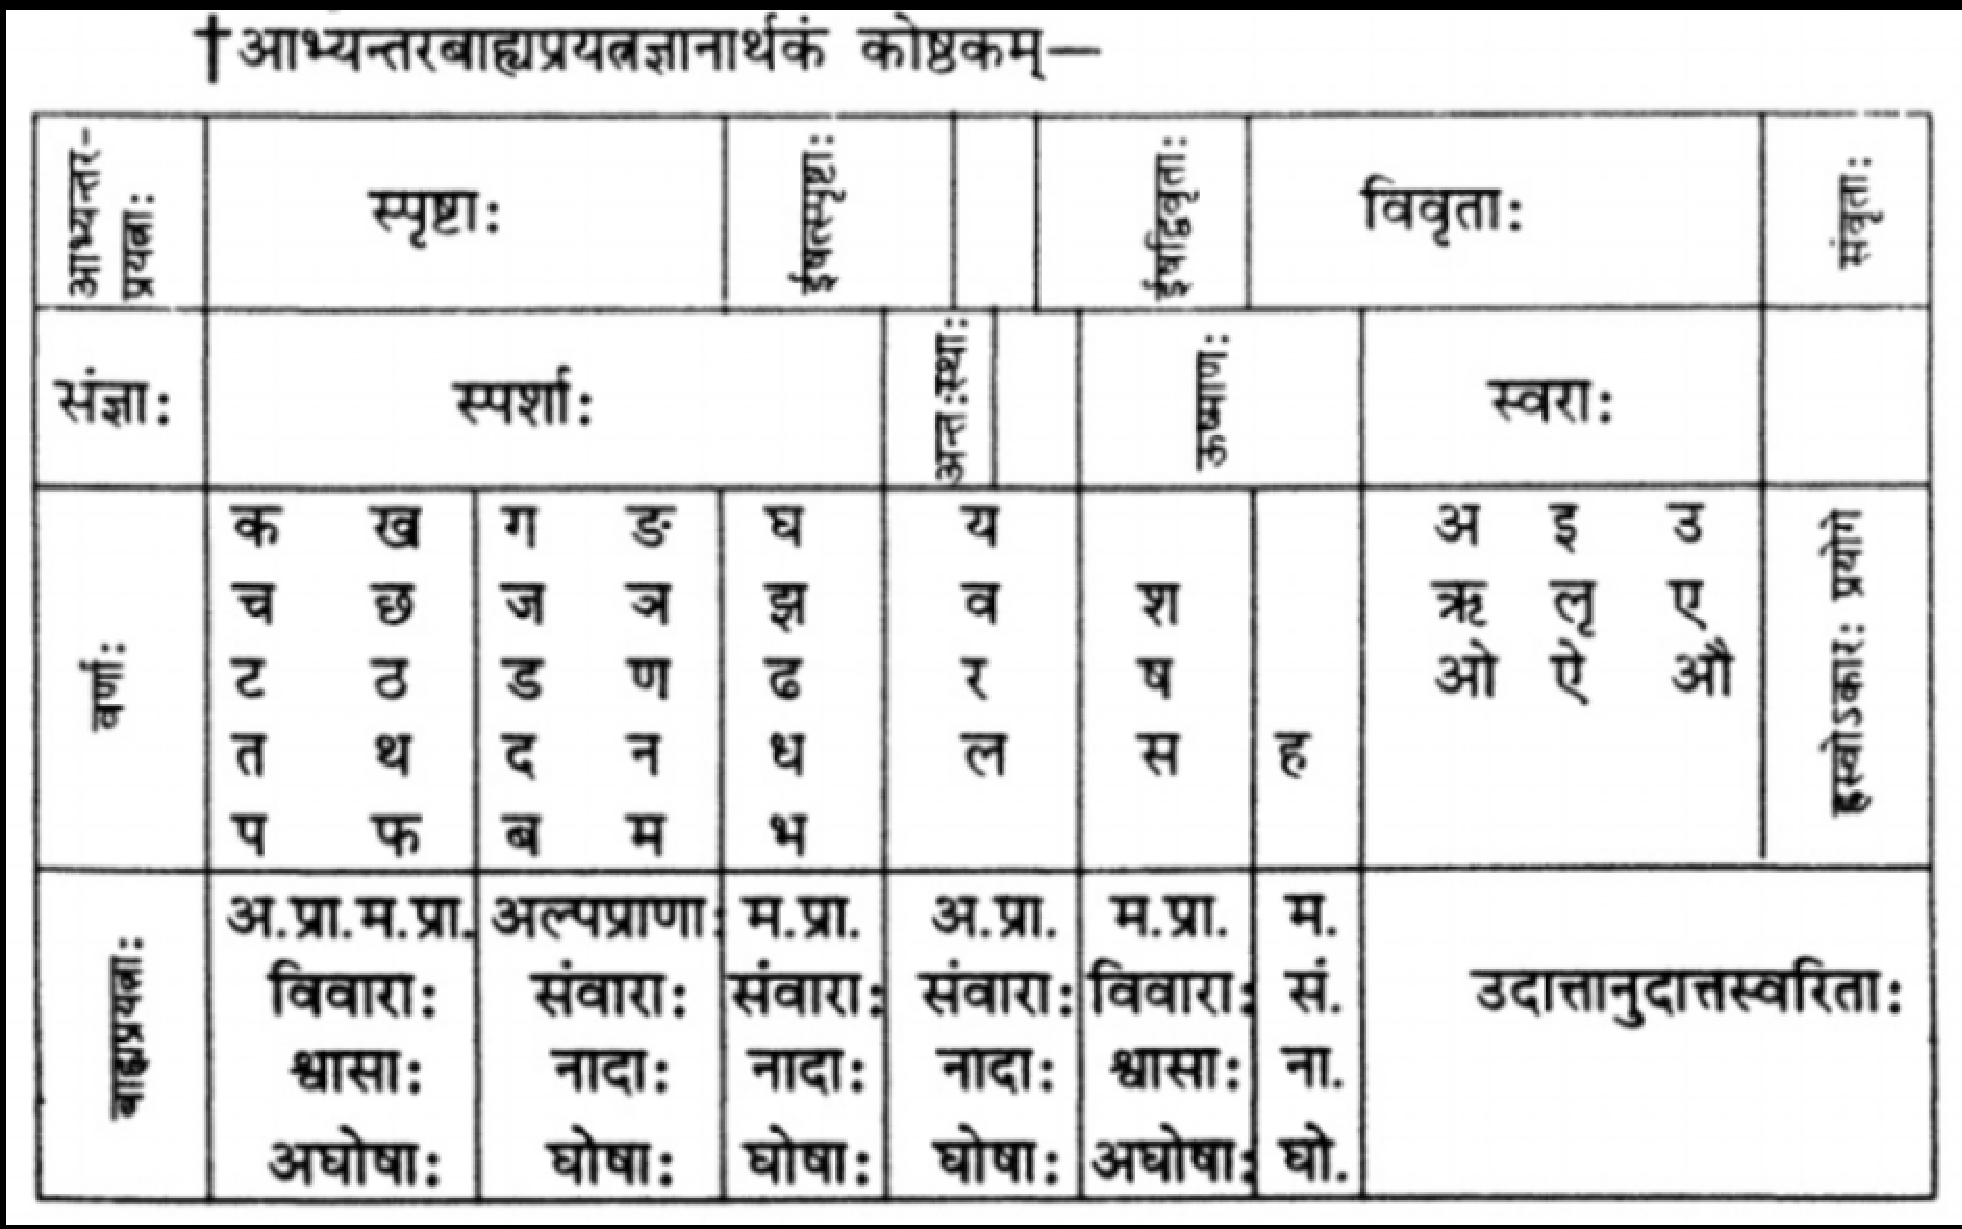
\includegraphics[scale=0.93]{"images/article-01/fig1.png"}\\Fig.~6.1 British Colonial Evangelical Construction of Encouraged Dravidian Identity
\end{center}

\newpage


\subsubsection*{De-Indianizing and Christianizing Āgama (Tamil spiritual traditions)}

\begin{center}
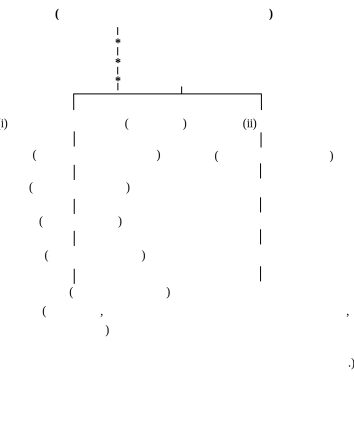
\includegraphics[scale=0.93]{"images/article-01/fig2.png"}\\Fig.~6.2 De-Indianizing and Christianizing Tamil Spiritual Traditions
\end{center}


\subsubsection*{Digesting Dharma into Dravidian Christianity}

\begin{center}
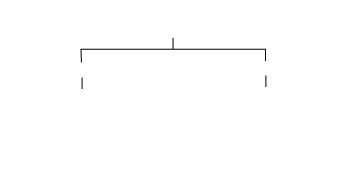
\includegraphics{"images/article-01/fig3.png"}\\Fig.~8.1 Preparing the Stage for Digestion of Hinduism into `Dravidian' Christianity
\end{center}


\subsubsection*{Western institutional control of social discourse in India}

\begin{center}
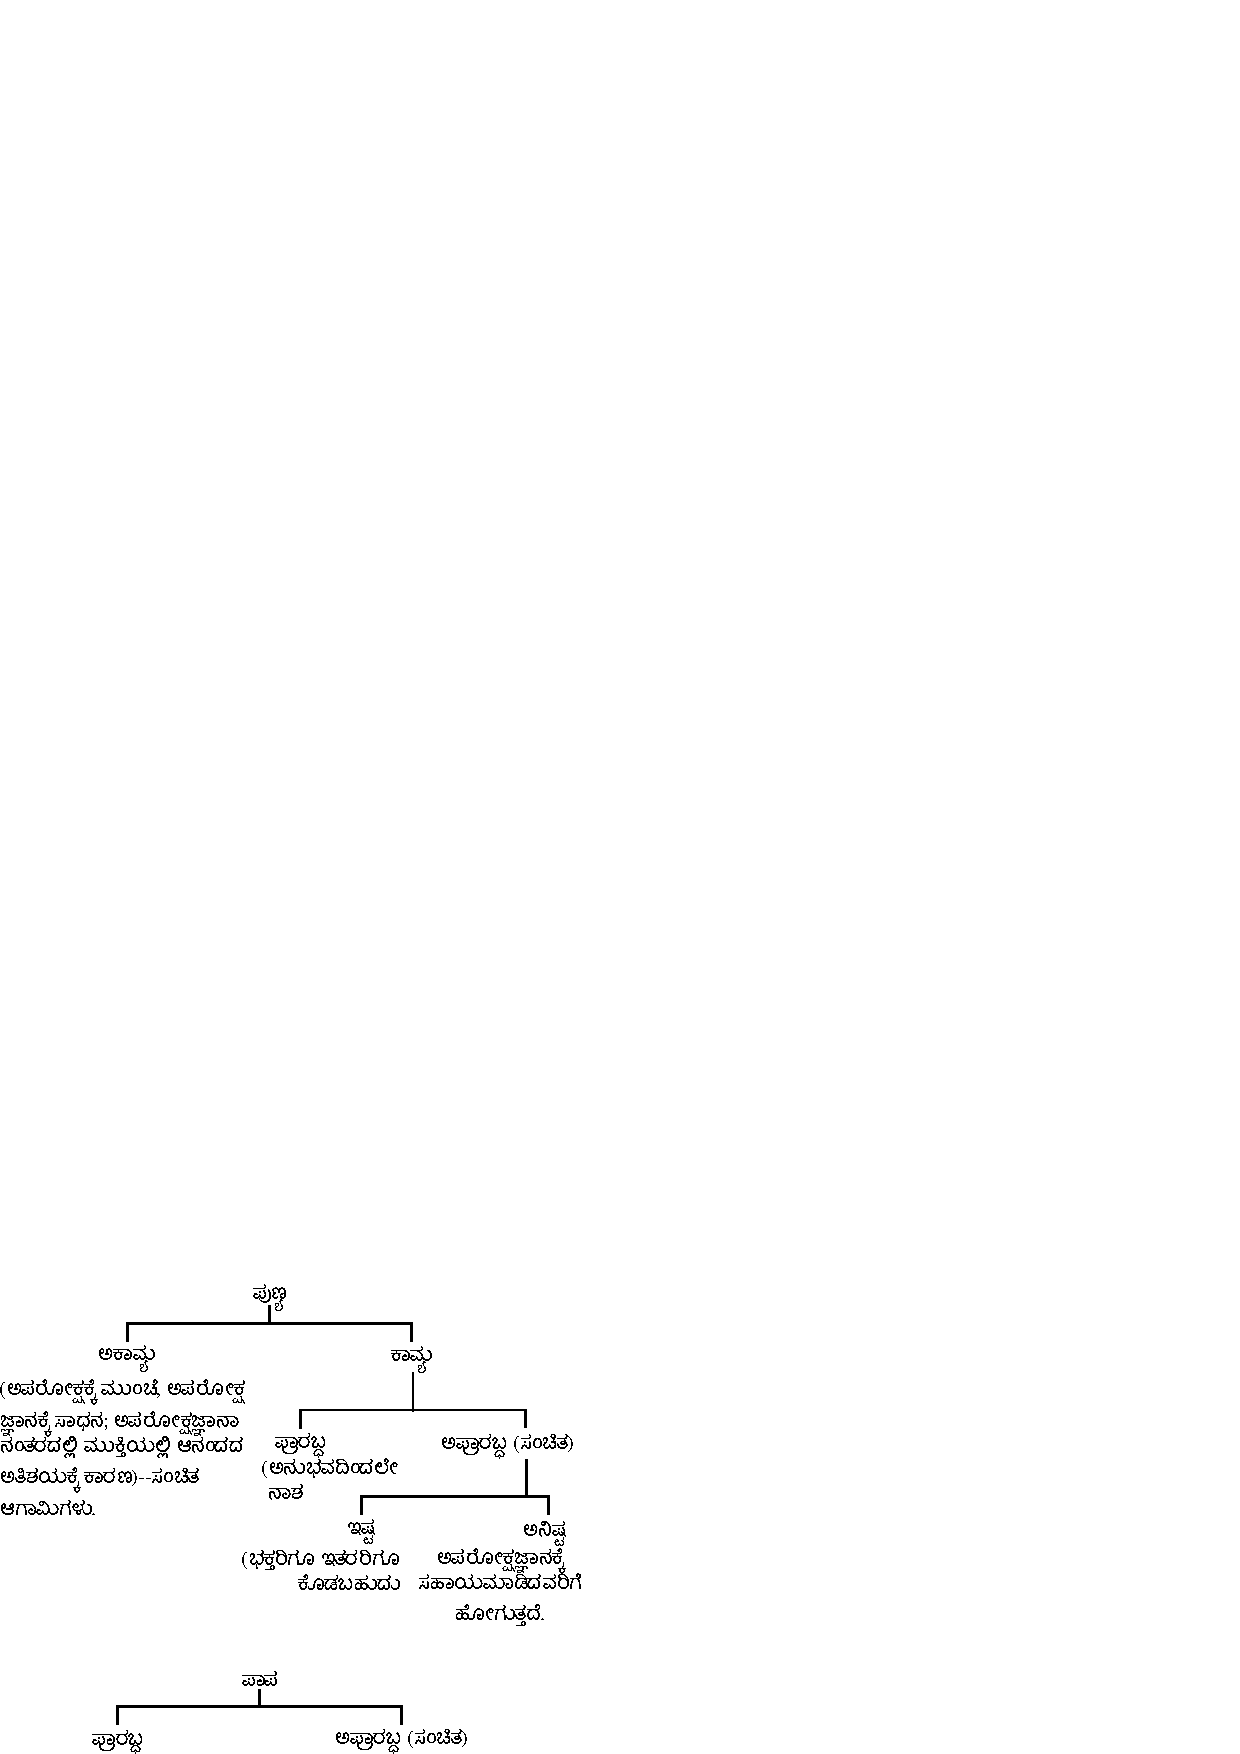
\includegraphics[scale=1.1]{"images/article-01/fig4.png"}\\Fig.~11.1 Western Institutional Control of Social Discourse in India
\end{center}


\subsubsection*{Western gaze on India: secular and biblical}

\begin{center}
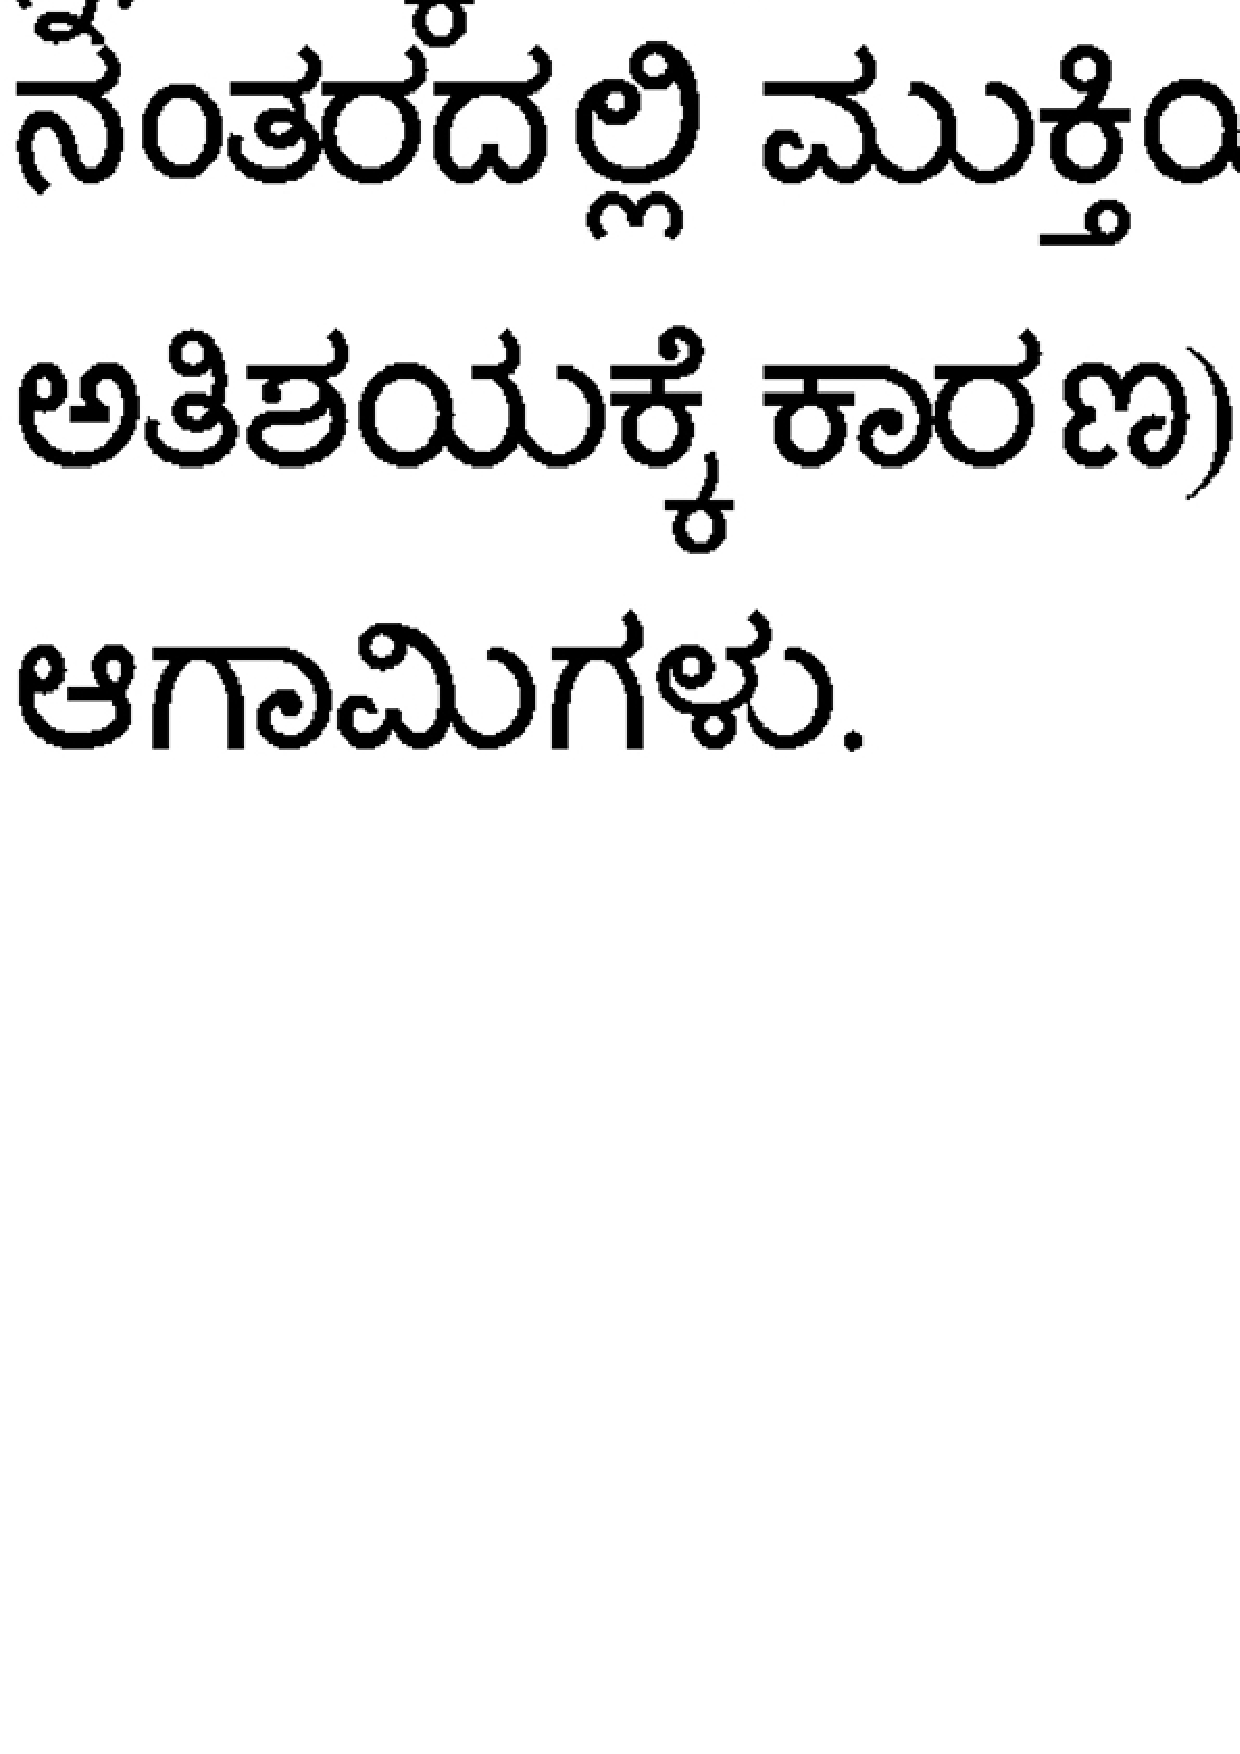
\includegraphics[scale=1.1]{"images/article-01/fig5.png"}\\Fig.~11.2 Western Perception of India Through Two Powerful Lenses
\end{center}

\newpage


\subsubsection*{Western academic manipulation of Dravidian identity}

\begin{center}
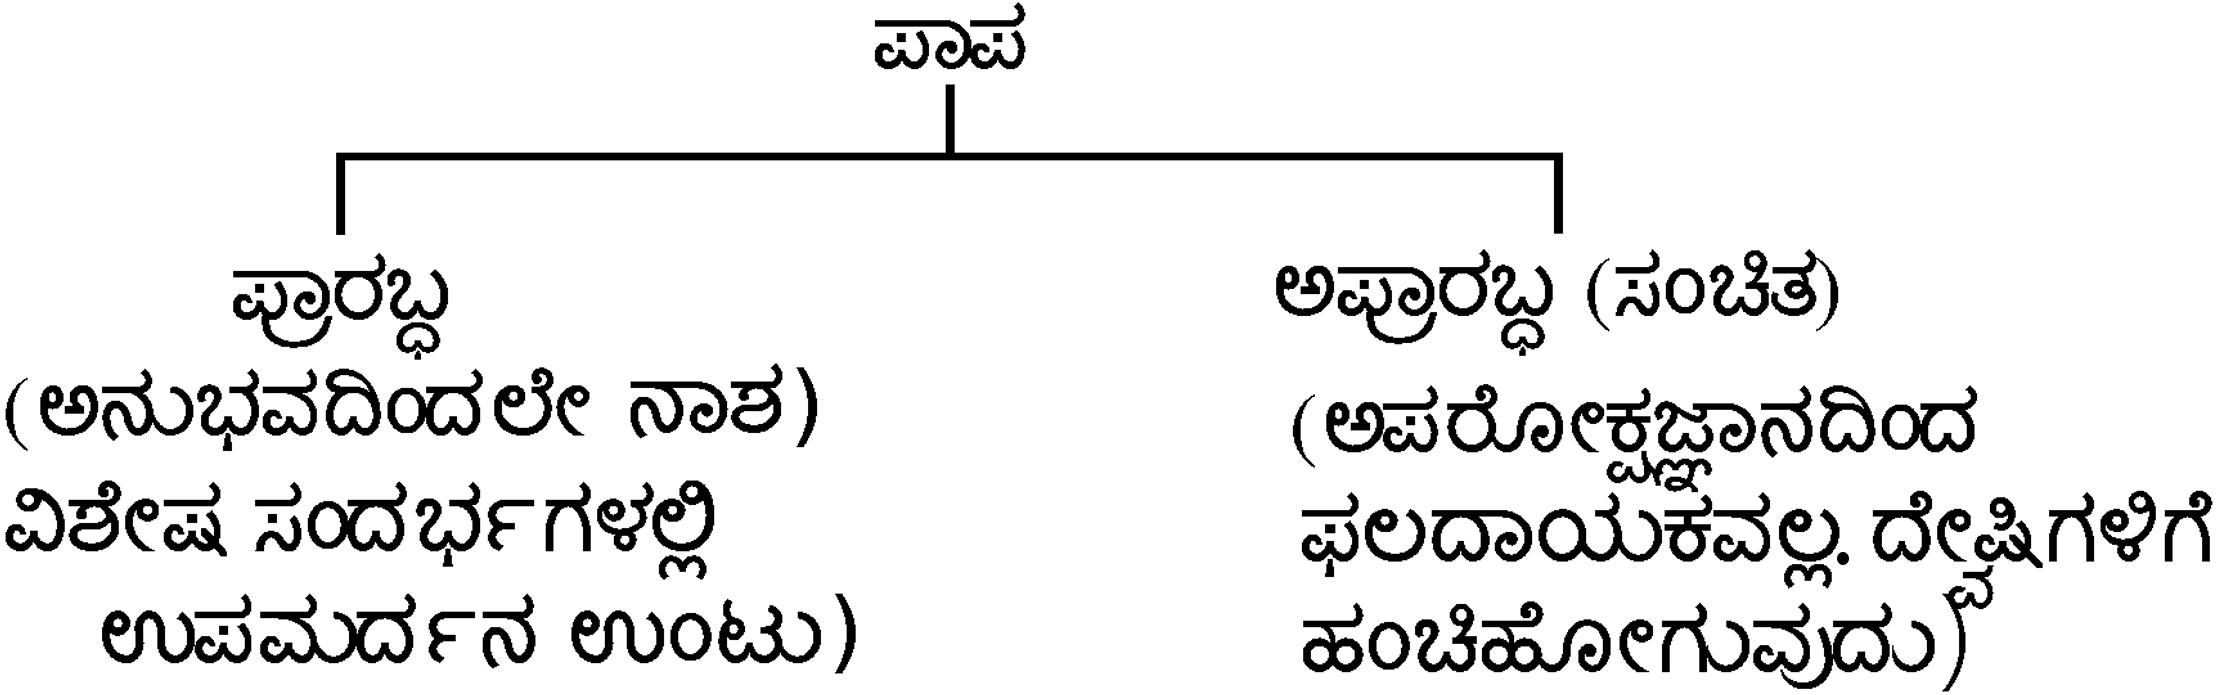
\includegraphics{"images/article-01/fig6.png"}\\Fig.~11.3 Academic Disciplines and Dravidian Identity Implications
\end{center}

\vskip 8pt



\section*{Bibliography}

\begin{thebibliography}{99}
\bibitem{chap3-key01} Bhikşu, Gauriśankara. 1950 (Samvat 2006; 6th ed). \textit{Sarvatantrasiddhāntapadārthalakşaņasangraha}. Kashi: Bhargava Bhushan Mudranalaya.

 \bibitem{chap3-key02} Ganesh, R and B.N. Shashi Kiran. 2017. “Debunking the Aryan-Dravidian Issue: An Indigenous Approach With special reference to three scholars from Karnataka.” Paper submitted at Swadeshi Indology III, Chennai 2017.

 \bibitem{chap3-key03} Gautier, Fançois. 2002. Marxism and Saffron Wave. www.rediff.com accessed on Dec 22, 2016. 

 \bibitem{chap3-key04} Jha, Girish Nath (2013), “Some remarks on the Origin and Development of Indian Langauges and Linguistic Area.” In \textit{Perspectives on the Origin of Indian Civilization} edited by Angela Marcantonio and Girish Nath Jha, New Delhi: D.K. Printworld.

 \bibitem{chap3-key05} Joshi, Ravi and Yamuna Harshavardhana. 2017 “Dravidianism with Language equaling Race -The third wheel in Tamil Sanskrit interactions.:” Paper submitted at Swadeshi Indology III, Chennai 2017.

 \bibitem{chap3-key06} Kazanas, N.2006. “Indo-Aryan indigenism and the Aryan Invasion Theory arguments (refuted).” \textit{Omilos Meleton}, Athens. \url{http://www.omilosmeleton.gr/pdf/en/indology/IIAR.pdf}); accessed May 2, 2018

 \bibitem{chap3-key07} Lele, W.K. 1981. \textit{The Doctrine of the Tantrayukti}-s. Waranasi: Chaukamba Surabharati Prakashan.

 \bibitem{chap3-key08} Malhotra, Rajiv and Aravindan Neelakandan. 2011. \textit{Breaking India: Western Interventions in Dravidian and Dalit Faultlines}. New Delhi: Amaryllis.

 \bibitem{chap3-key09} Ouseparampil, J. (trans). 1990. “Indian Aesthetics and Hermeneutics." \textit{Indian Journal of Spirituality}, Vol. Ill, 2 (Bangalore: Fransalian Institute of Spirituality (1990).

 \bibitem{chap3-key10} Prithipaul, K. Dad. 2005. “Hindu Dharma and Indian Funk.” In \textit{Dharma The Categorial Imperative}, edited by Arvind Sharma, Ashok Vohra, Mrinal Miri. Delhi: D. K. Printworld.

 \bibitem{chap3-key11} Risley, Herbert. The People of India. London. W. Thacker and Co., 1915.

 \bibitem{chap3-key12} Sri Sri Ravi Shankar. 2005. “Stick to your ground.” Pune: \textit{The Times of India}, November 5, 2005.

 \bibitem{chap3-key13} Wakankar, V. S. 2008. \textit{Indian Prehistory as Revealed by Excavations, Explorations and Rock Art Study at Bhimbetka and in the Adjoining Regions}. Purakala. 

 \end{thebibliography}

